\section{Mobile CI/CD}

Coming now from the "classical" CI/CD approach, it is not possible to instantly apply the known model to the mobile world, it needs some adoption. Before we do so, we have to consider the following points: \\

\begin{itemize}
	
	\item \textbf{Mobile application have a high UI focus} \\
	UI tests are always more expensive to create than for "standard" code - and this is even more valid for mobile applications. Additionally from the known challenges of desktop applications like clickable fields, listener states, dependencies between views \& co, a mobile device introduces complexity
	\\
	
	\item \textbf{Mobile applications have per default a build tool} \\
	Both iOS (\textit{XCode}) and Android (\textit{AndroidStudio} \& \textit{gradle}) come along with their own build system and IDE, making the question if the application is build manually or automated with a tool pointless.
	\\
	
	\item \textbf{There is no standard production environment} \\
	Due to the nature of the mobile device world, there is no standard device towards a deployment can happen. Especially but not only with Android there is a huge variety of screen sizes and operating system versions to be handled. Therefore automated testing has to be a compromise between covered variations and invested efforts. There are of course attempts to test with assuming the maximum coverage of variations, but it can never be sufficient as for e.g. a server software.
	\\
	
	\item \textbf{Emulation is expensive} \\
	Another consequence of the variety of device types, testing with real hardware is a pain and lead to the usage of emulators. But emulation is expensive in terms of time and resources, especially since due to the high share of required UI tests, a majority of testing can not be done independent from the (emulated) mobile OS.
	
\end{itemize}

\subsection{Adopted CI/CD model}
As consequence to the mentioned points, we will adopt the practise checklist of Fowler by completely removing 2) (inherited to the build tools) and changing 7) to "Test in a Emulated Environment".

\subsection{Googles CI/CD tools}

Google provides many frameworks and guidelines which can be pretty overwhelming - this and the next section is therefore dedicated to give an overview of these and summarize which options there are to implement a proper CI/CD pipeline within the Android world. 

\subsubsection{Android Emulator}

Bundled within the Android SDK comes the Android Emulator\footnote{\url{https://developer.android.com/studio/run/emulator}}, which allows the emulation of a virtual device on the local machine. It supports various images, called Android Virtual Devices (AVD), with different configuration options. Once launched it is considered as a real device by \texttt{adb} and can therefore used as deployment target. The tool further provides the option to launch without an UI and to be used for testing on a server.

\subsubsection{Firebase Test Lab}
With Firebase Test Lab\footnote{\url{https://firebase.google.com/docs/test-lab/android/overview}} Google offers a cloud-based device farm with virtual and real devices. It supports two different testing methods: Instrumentation (see section~\ref{sec:test_types}) and Robo (basic test type that simulates real user interactions) Tests. Test results are provided with additional logs, videos and screenshots.
Firebase Test Lab allows 10 tests per day for virtual devices and 5 for physical devices in it's free version ("Spark Plan") - but some CI/CD cloud services like Bitrise included the service within their contingents.

\subsubsection{Google Play Deploy}
Google offers via the Play Store console a REST API to deploy compiled APKs and AABs which can be used in an CD setup. The API is secured via the according Service account. Additionally to the (not prefered way) direct release track it is possible to deploy to the \texttt{alpha}, \texttt{beta} or \texttt{internal} tracks\footnote{\url{https://developers.google.com/android-publisher/tracks}}.

\subsubsection{Available CI/CD Server}

In order to properly utilize a mobile CI/CD pipeline there are many estabilshed server provider around - since it would exceed the scope of this paper to make a full comparison of these service providers, we limit it to a selection of the most commons:

\begin{itemize}
	\item Bitrise\footnote{\url{https://www.bitrise.io/}}
	\item TeamCity\footnote{\url{https://www.jetbrains.com/teamcity/}}
	\item Travis CI\footnote{\url{https://travis-ci.org/}}
	\item Jenkins\footnote{\url{https://jenkins.io/}}
	\item Bamboo\footnote{\url{https://www.atlassian.com/software/bamboo}}
	\item GitLab CI/CD\footnote{\url{https://about.gitlab.com/product/continuous-integration/}}
	\item CircleCI\footnote{\url{https://circleci.com/}}
\end{itemize}

\subsection{Android testing}

\begin{figure}[htb]
	\centering
	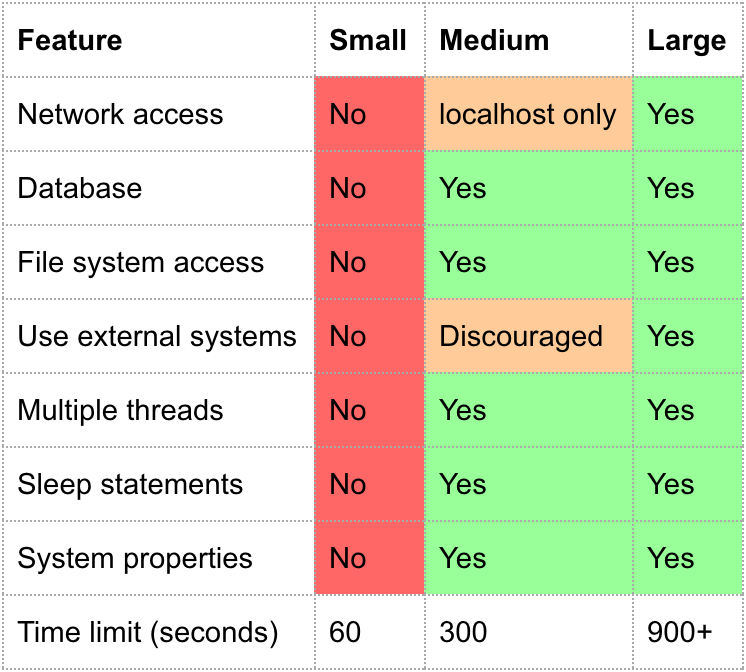
\includegraphics[width=0.5\textwidth]{./test_sizes.png}
	\caption[Test Sizes]{Test Sizes\footnotemark}
	\label{fig_google_test_sizes}
\end{figure}
\footnotetext{\url{https://testing.googleblog.com/2010/12/test-sizes.html}}

\begin{itemize}
	\item \textbf{Small tests} \\ 
	70\% unit tests, JUnit, Mockito, PowerMock
	
	\item \textbf{Medium tests} \\ 
	 20\% Integration Tests, Robolectric
	 
	\item \textbf{Large tests} \\ 
	 10\% UI Test, Espresso, Robotium, UI Automator
\end{itemize}

\subsubsection{Local tests VS device tests}\label{sec:test_types}

\texttt{test} for unit tests, run on local machine/JVM \\
\texttt{androidTest} for instrumented tests, integration tests, UI tests

\subsubsection{AndroidJUnit4}
\textbf{Android JUnit Runner} \\
\textbf{Android Test Orchestrator}

\subsubsection{UI Automator}
\subsubsection{Espresso}
\subsubsection{Robolectric}
\subsubsection{Android Jetpack Test}

\begin{mdframed}[style=InfoBox,align=center]
	\textbf{Note:} Google recently (I/O18) announced "Project Nitrogen" which intents to remove any restrictions of tests to run time environment - but there are no more information available at time of writing this paper.
\end{mdframed}

\begin{figure}[htb]
	\centering
	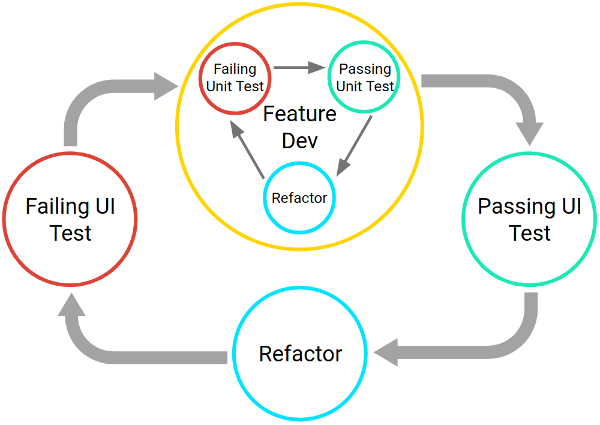
\includegraphics[width=0.5\textwidth]{./google_testing.png}
	\caption[The two cycles associated with iterative, test-driven development]{The two cycles associated with iterative, test-driven development\footnotemark}
	\label{fig_google_testing}
\end{figure}
\footnotetext{\url{https://developer.android.com/images/training/testing/testing-workflow.png}}

\begin{figure}[htb]
	\centering
	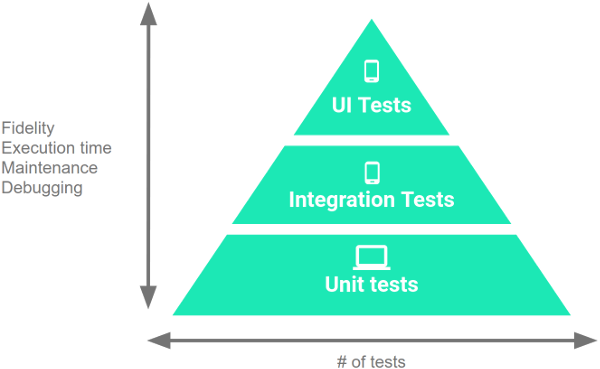
\includegraphics[width=0.5\textwidth]{./pyramid.png}
	\caption[The Testing Pyramid, showing the three categories of tests that should be included in an app's test suite]{The Testing Pyramid, showing the three categories of tests that should be included in an app's test suite\footnotemark}
	\label{fig_google_pyramid}
\end{figure}
\footnotetext{\url{https://developer.android.com/images/training/testing/pyramid.png}}
